\documentclass[12pt]{article}

% You need graphics package
\usepackage{color}
\usepackage{graphicx}
\usepackage{pst-all}
\usepackage{advi}
\pagestyle{empty}

\definecolor{red}{rgb}{1.0,0.0,0.0}
\definecolor{salmon}{rgb}{1.0,0.8,0.8}
\definecolor{green}{rgb}{0.8,1.0,0.8}
\definecolor{blue}{rgb}{0.8,0.8,1.0}
\definecolor{yellow}{rgb}{1.0,1.0,0.8}
\definecolor{magenta}{rgb}{1.0,0.8,1.0}
\definecolor{cyan}{rgb}{0.8,1.0,1.0}

\def\smallpause{0.3}

\def\keymenu#1{\textcolor{red}{\underline{#1}}}

\def\advifooter{\vbox to 0em{\vbox to \vsize {\vfill
Press: %
\keymenu{n}ext page %
\keymenu{p}revious page %
\keymenu{\textvisiblespace} next pause%
\hfill\vspace*{-0.6cm}{\adviembed[sticky=advianim,width=1.56cm,height=1.824cm]%
{animate -geometry @g! -window @p advilogo.anim.gif}}
}
\vss}}

\def\adviheader{\noindent
{\bf\Large {\ActiveDVI}  --- transitions}\\

\includegraphics[width=\textwidth]{bar.eps}}

\def\pstricksback#1{%
\hspace{-\textwidth}%
\rput(-0.7cm,-0.5cm){\psframe[framearc=.1,fillstyle=solid,linestyle=none,fillcolor=#1](1.1\textwidth,-0.85\textheight)}
}

\let\Newpage\newpage
\def\newpage{\Newpage\advifooter\adviheader}

\def\adviemptyfooter{\vbox to 0em{\vbox to \vsize {\vfill
~~} \vss\advikillembed{advianim}}}

\def\lastpage{\Newpage\adviemptyfooter\adviheader}

%  \setlength\textwidth{660\p@}
%  \setlength\textheight{460\p@}

\begin{document}

\newpage\pstricksback{salmon}

\subsection*{Transitions}

{\ActiveDVI} has transitions --- animated page display for each pause.
You can specify the transition by \verb|\advitransition{|%
$mode~arg_1~\ldots~arg_n$\verb|}| advi macro.
Currently the following transition modes are available:
\begin{itemize}
\item {\tt none } --- no transition animation
\item {\tt slide} --- new page slides on the screen
\item {\tt wipe } --- new page wipes on the screen
\item {\tt block} --- new page is split into small pieces and they
appear randomly
\end{itemize}
For example, if you want to slide the page, write
\verb+\advitransition{slide}+ in your document. 

\subsection*{Notes}

\begin{itemize}
\item The transition state of advi is currently reset to \verb|none|
  at the beginning of each page.
\item The transition animations occur even at \verb+\pause+ and
  \verb+\wait+ commands. 
  If you feel it too lousy for each pause, 
  you have to disable the transition by \verb+\advitransition{none}+
  just before pauses.
\end{itemize}

\newpage\pstricksback{green}

\subsection*{Transitions parameters}
Each transition mode has additional parameters to control its details. 
Usually the followings are available:
\begin{itemize}
\item {\tt from=}{\em{arg}} --- new pages come from the direction of
  {\em arg} (\verb+left+, \verb+right+, \verb+top+, \verb+bottom+,
\verb+topleft+, etc)
\item {\tt steps=}{\em{arg}}  --- number of animation steps
\end{itemize}
For example, if you want to slide-in a page from left in 30 steps,
write \verb+\advitransition{slide, from=left, steps=30}+.

\newpage\pstricksback{blue}

\subsection*{Slide transition}
\advitransition{slide, from=topleft, steps=30}
New pages appears sliding into the screen.

\subsubsection*{Options}
\begin{itemize}
\item {\tt from=}{\em{arg}} --- new pages come from the direction of
  {\em arg} (one of \verb+left+, \verb+right+, \verb+top+,
  \verb+bottom+, \verb+topleft+, \verb+topright+, \verb+bottomleft+,
  \verb+bottomright+). The default is \verb+right+.
\item {\tt steps=}{\em{arg}}  --- animation steps. The default is \verb+20+.
\end{itemize}

\subsubsection*{Examples}
\begin{itemize}
\item \verb+\advitransition{slide}+
\item \verb+\advitransition{slide, from=left, steps=30}+
\end{itemize}

\begin{flushright}
\epstransparent
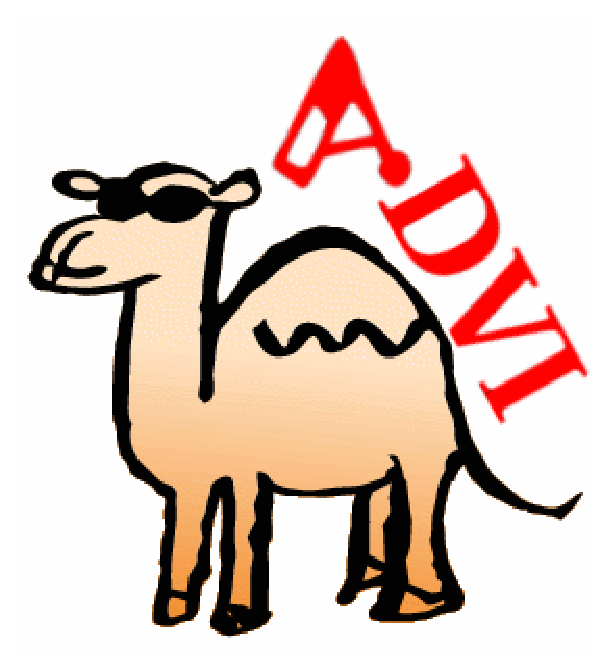
\includegraphics[width=0.25\textwidth]{../tex/advilogo.eps}
\end{flushright}

\newpage\pstricksback{yellow}

\advitransition{wipe, from=right, steps=30}

\subsection*{Wipe transition}
New pages appears wiping out the old graphics.

\subsubsection*{Options}
\begin{itemize}
\item {\tt from=}{\em{arg}} --- new pages come from the direction of
  {\em arg} (one of \verb+left+, \verb+right+, \verb+top+,
  \verb+bottom+, \verb+topleft+, \verb+topright+, \verb+bottomleft+,
  \verb+bottomright+, \verb+center+). The default is \verb+right+.
\item {\tt steps=}{\em{arg}}  --- animation steps. The default is \verb+20+.
\end{itemize}

\subsubsection*{Examples}
\begin{itemize}
\item \verb+\advitransition{wipe}+
\item \verb+\advitransition{wipe,from=center,steps=30}+
\end{itemize}

\begin{flushleft}
\epstransparent
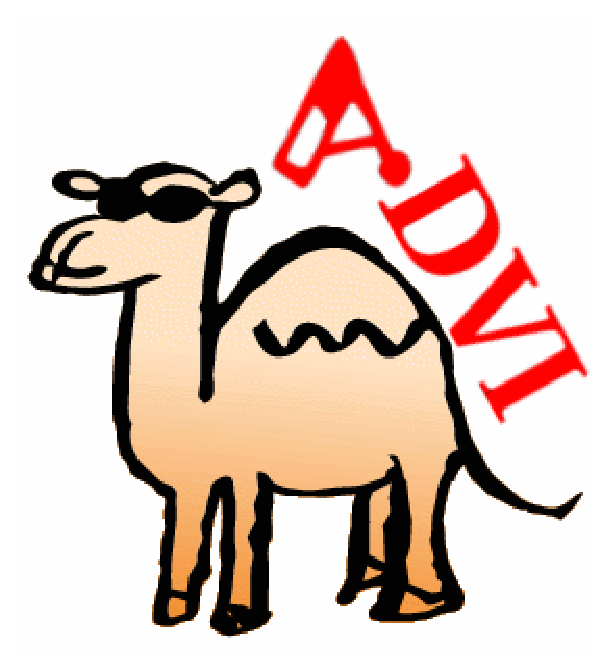
\includegraphics[width=0.25\textwidth]{../tex/advilogo.eps}
\end{flushleft}

\newpage\pstricksback{magenta}
\advitransition{block,from=topleft,steps=500}

\subsection*{Block transition}
New pages appears gradually into small pieces.

\subsubsection*{Options}
\begin{itemize}
\item {\tt from=}{\em{arg}} --- new pages come from the direction of
  {\em arg} (one of \verb+left+, \verb+right+, \verb+top+,
  \verb+bottom+, \verb+topleft+, \verb+topright+, \verb+bottomleft+,
  \verb+bottomright+, \verb+center+). The default is \verb+right+.
\item {\tt steps=}{\em{arg}}  --- number of blocks. The default is \verb+5000+.
\end{itemize}

\subsubsection*{Examples}
\begin{itemize}
\item \verb+\advitransition{block}+
\item \verb+\advitransition{block,from=topleft,steps=1000}+
\end{itemize}

\begin{flushright}
\epstransparent
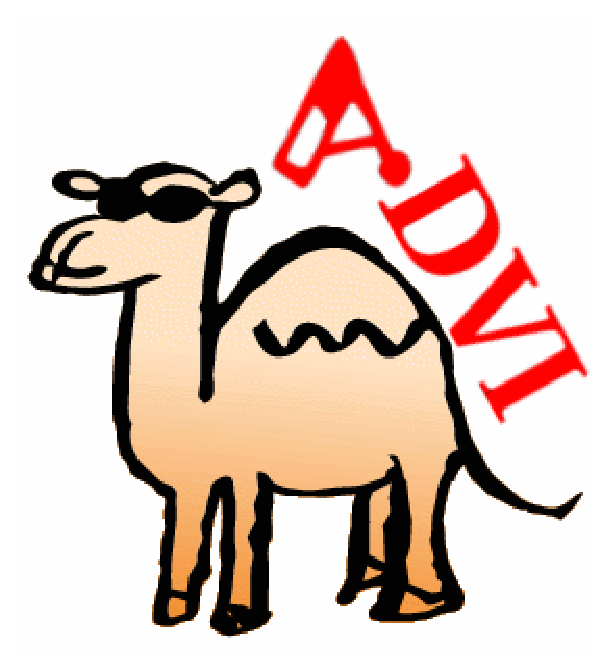
\includegraphics[width=0.25\textwidth]{../tex/advilogo.eps}
\end{flushright}

\lastpage

\advitransition{block,from=center,steps=500}

\adviwait[0.1]

~\vfill
\begin{center}
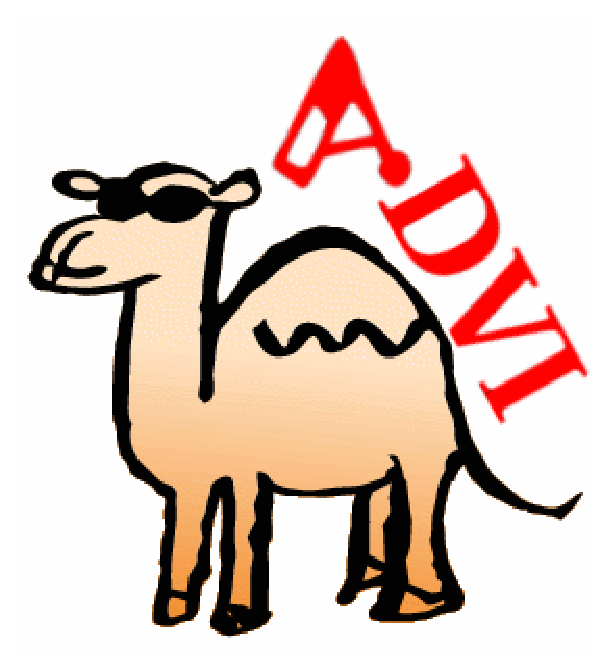
\includegraphics[width=0.5\textwidth]{../tex/advilogo.eps}\\
\adviwait[0.1]
\bigskip
{\Huge \bf That's all, folks!!}
\end{center}
~\vfill


\end{document}
